\documentclass[11pt,a4paper,serbian,oneside]{book}
\usepackage[utf8]{inputenc}
\usepackage[T1, T2A]{fontenc}
\usepackage{amsmath}
\usepackage{amssymb}
\usepackage{textcomp}
\usepackage{amsfonts}
\usepackage{graphicx}
\usepackage{ucs}
\usepackage{listings}
\usepackage[serbianc]{babel}
\usepackage{pdfsync}
\usepackage[left=2.5cm,right=2.5cm,top=2.5cm,bottom=2.5cm]{geometry}
\usepackage{float}
\usepackage{wrapfig}
\usepackage{color}
\usepackage{xcolor}
\usepackage{caption}
\usepackage{subcaption}
\usepackage{nameref}
\usepackage{url}

% Definisanje boja
\definecolor{lightgray}{rgb}{0.95, 0.95, 0.95}
\definecolor{darkgray}{rgb}{0.4, 0.4, 0.4}
\definecolor{purple}{rgb}{0.65, 0.12, 0.82}
\definecolor{ocherCode}{rgb}{1, 0.5, 0} % #FF7F00 -> rgb(239, 169, 0)
\definecolor{blueCode}{rgb}{0, 0, 0.93} % #0000EE -> rgb(0, 0, 238)
\definecolor{greenCode}{rgb}{0, 0.6, 0} % #009900 -> rgb(0, 153, 0)

\colorlet{punct}{red!60!black}
%\definecolor{background}{HTML}{EEEEEE}
\definecolor{delim}{RGB}{20,105,176}
\colorlet{numb}{magenta!60!black}

% Komanda za horizontal ruler
\newcommand{\HRule}{\rule{\linewidth}{0.5mm}}

%
% Definicija fiksiranih reci
%
\addto\captionsserbian{%
 \def\prefacename{Предговор}%
 \def\refname{Списак литературе}%
 \def\abstractname{Сажетак}%
 \def\bibname{Литература}%
 \def\chaptername{Глава}%
 \def\appendixname{Додатак}%
 \def\contentsname{Садржај}%
 \def\listfigurename{Списак слика}%
 \def\listtablename{Списак табела}%
 \def\indexname{Регистар}%
 \def\figurename{Слика}%
 \def\tablename{Табела}%
 \def\partname{Део}%
 \def\enclname{Прилози}%
 \def\ccname{Копије}%
 \def\headtoname{Прима}%
 \def\pagename{Страна}%
 \def\seename{Види}%
 \def\alsoname{Види такође}%
 \def\proofname{Доказ}%
 \def\glossaryname{Речник непознатих речи}
 \def\contentsname{Садржај}%
 }%

%
% Podesavanja paketa za listinge
%
\renewcommand\lstlistingname{Листинг}

\makeatletter
\newcommand*{\srb}[1]{%
  \expandafter\@srb\csname c@#1\endcsname
}
\newcommand*{\@srb}[1]{%
  \ifcase#1\or a\or б\or в\or г\or д\or ђ\or е\or ж\or з\or и\or ј%
    \or к\or л\or љ\or м\or н\or њ\or о\or п\or р\or с\or т\or ћ%
    \or у\or ф\or х\or ц\or ч\or џ\or ш%
    \else\@ctrerr\fi
}

\renewcommand{\thesubfigure}{\srb{subfigure}}

\lstdefinelanguage{CSS}{
  morekeywords={accelerator,azimuth,background,background-attachment,
    background-color,background-image,background-position,
    background-position-x,background-position-y,background-repeat,
    behavior,border,border-bottom,border-bottom-color,
    border-bottom-style,border-bottom-width,border-collapse,
    border-color,border-left,border-left-color,border-left-style,
    border-left-width,border-right,border-right-color,
    border-right-style,border-right-width,border-spacing,
    border-style,border-top,border-top-color,border-top-style,
    border-top-width,border-width,bottom,caption-side,clear,
    clip,color,content,counter-increment,counter-reset,cue,
    cue-after,cue-before,cursor,direction,display,elevation,
    empty-cells,filter,float,font,font-family,font-size,
    font-size-adjust,font-stretch,font-style,font-variant,
    font-weight,height,ime-mode,include-source,
    layer-background-color,layer-background-image,layout-flow,
    layout-grid,layout-grid-char,layout-grid-char-spacing,
    layout-grid-line,layout-grid-mode,layout-grid-type,left,
    letter-spacing,line-break,line-height,list-style,
    list-style-image,list-style-position,list-style-type,margin,
    margin-bottom,margin-left,margin-right,margin-top,
    marker-offset,marks,max-height,max-width,min-height,
    min-width,-moz-binding,-moz-border-radius,
    -moz-border-radius-topleft,-moz-border-radius-topright,
    -moz-border-radius-bottomright,-moz-border-radius-bottomleft,
    -moz-border-top-colors,-moz-border-right-colors,
    -moz-border-bottom-colors,-moz-border-left-colors,-moz-opacity,
    -moz-outline,-moz-outline-color,-moz-outline-style,
    -moz-outline-width,-moz-user-focus,-moz-user-input,
    -moz-user-modify,-moz-user-select,orphans,outline,
    outline-color,outline-style,outline-width,overflow,
    overflow-X,overflow-Y,padding,padding-bottom,padding-left,
    padding-right,padding-top,page,page-break-after,
    page-break-before,page-break-inside,pause,pause-after,
    pause-before,pitch,pitch-range,play-during,position,quotes,
    -replace,richness,right,ruby-align,ruby-overhang,
    ruby-position,-set-link-source,size,speak,speak-header,
    speak-numeral,speak-punctuation,speech-rate,stress,
    scrollbar-arrow-color,scrollbar-base-color,
    scrollbar-dark-shadow-color,scrollbar-face-color,
    scrollbar-highlight-color,scrollbar-shadow-color,
    scrollbar-3d-light-color,scrollbar-track-color,table-layout,
    text-align,text-align-last,text-decoration,text-indent,
    text-justify,text-overflow,text-shadow,text-transform,
    text-autospace,text-kashida-space,text-underline-position,top,
    unicode-bidi,-use-link-source,vertical-align,visibility,
    voice-family,volume,white-space,widows,width,word-break,
    word-spacing,word-wrap,writing-mode,z-index,zoom},
  morestring=[s]{:}{;},
  sensitive,
  morecomment=[s]{/*}{*/}
}

\lstdefinelanguage{HTML5}{
    sensitive=true,
    keywords={%
    % JavaScript
    typeof, new, true, false, catch, function, return, null, catch, switch, var, if, in, while, do, else, case, break,
    % HTML
    html, title, meta, style, head, body, script, canvas, div
    % CSS
    border:, transform:, -moz-transform:, transition-duration:, transition-property:,
    transition-timing-function:
    },
    % http://texblog.org/tag/otherkeywords/
    otherkeywords={<, >, \/},
    ndkeywords={class, export, boolean, throw, implements, import, this},
    comment=[l]{//},
    % morecomment=[s][keywordstyle]{<}{>},
    morecomment=[s]{/*}{*/},
    morecomment=[s]{<!}{>},
    morestring=[b]',
    morestring=[b]",
    alsoletter={-},
    alsodigit={:}
}

\lstdefinelanguage{json}{
    basicstyle=\fontsize{9}{11}\ttfamily,
    numbers=left,
    numberstyle=\scriptsize,
    stepnumber=1,
    numbersep=8pt,
    showstringspaces=false,
    breaklines=true,
    frame=lines,
    %backgroundcolor=\color{background},
    literate=
     *{0}{{{\color{numb}0}}}{1}
      {1}{{{\color{numb}1}}}{1}
      {2}{{{\color{numb}2}}}{1}
      {3}{{{\color{numb}3}}}{1}
      {4}{{{\color{numb}4}}}{1}
      {5}{{{\color{numb}5}}}{1}
      {6}{{{\color{numb}6}}}{1}
      {7}{{{\color{numb}7}}}{1}
      {8}{{{\color{numb}8}}}{1}
      {9}{{{\color{numb}9}}}{1}
      {:}{{{\color{punct}{:}}}}{1}
      {,}{{{\color{punct}{,}}}}{1}
      {\{}{{{\color{delim}{\{}}}}{1}
      {\}}{{{\color{delim}{\}}}}}{1}
      {[}{{{\color{delim}{[}}}}{1}
      {]}{{{\color{delim}{]}}}}{1},
}

\lstset {
	basicstyle=\fontsize{9}{11}\ttfamily,
	numbers=left,
	numberstyle=\tiny,
	%stepnumber=2,
	numbersep=5pt,
	extendedchars=true,
	breaklines=true,
	keywordstyle=\color{blue},
	frame=b,
    % Code design
	stringstyle=\color{white}\ttfamily,
    identifierstyle=\color{black},
    keywordstyle=\color{blue}\bfseries,
    ndkeywordstyle=\color{greenCode}\bfseries,
    commentstyle=\color{darkgray}\ttfamily,
    % Code
	tabsize=2,
	showspaces=false,
	showtabs=false,
	xleftmargin=17pt,
	framexleftmargin=14pt,
	framexrightmargin=3pt,
	framexbottommargin=4pt,
	framextopmargin=0pt,
	%backgroundcolor=\color{lightgray},
	showstringspaces=false,
    extendedchars=true,
    breaklines=true	
}


\lstset{%
    % Basic design
    basicstyle=\fontsize{9}{11}\ttfamily,
    frame=l,
    % Line numbers
    xleftmargin={0.75cm},
    numbers=left,
    stepnumber=1,
    firstnumber=1,
    numberfirstline=true,
    % Code design
    identifierstyle=\color{black},
    keywordstyle=\color{blue}\bfseries,
    ndkeywordstyle=\color{greenCode}\bfseries,
    stringstyle=\color{ocherCode}\ttfamily,
    commentstyle=\color{darkgray}\ttfamily,
    % Code
    language={HTML5},
    tabsize=2,
    showtabs=false,
    showspaces=false,
    showstringspaces=false,
    extendedchars=true,
    breaklines=true
}

\lstloadlanguages {
	% Check Documentation for further languages ...
	%[Visual]Basic
	%Pascal
	C,
	%C++
	%Java,
	%XML,
	HTML5
}

%
% Podesavanje okvira listinga
%
\DeclareCaptionFont{white}{\color{white}}
\DeclareCaptionFormat{listing}{\colorbox[cmyk]{0.43, 0.35, 0.35,0.01}{\parbox{\textwidth}{\hspace{12pt}#1#2#3}}}
\captionsetup[lstlisting]{format=listing,labelfont=white,textfont=white, singlelinecheck=false, margin=0pt, font={bf,footnotesize} }


%
% Pocetak dokumenta
%
\begin{document}

%
% Naslovna stranica
%

\begin{titlepage}

\begin{center}

% Gornji deo stranice

\includegraphics[width=0.25\textwidth]{logo-pmf.pdf}\\[1cm]

\textsc{\LARGE Институт за математику и информатику
\\ Природно-математички факултет
\\ Универзитет у Крагујевцу}\\[1.5cm]

\textsc{\Large Дипломски рад}\\[0.5cm]

% Naslov
\HRule \\[0.4cm]
{ \huge \bfseries Синхронизација календара за \textit{оwnCloud} платформу}\\[0.4cm]

\HRule \\[1.5cm]

% Autor i mentor
\begin{minipage}{0.4\textwidth}
\begin{flushleft} \large
\emph{Студент:}\\
Владимир Варагић
\end{flushleft}
\end{minipage}
\begin{minipage}{0.4\textwidth}
\begin{flushright} \large
\emph{Професор:} \\
др Милош Ивановић
\end{flushright}
\end{minipage}

\vfill

% Dno stranice
{\large Август 2016.}

\end{center}

\end{titlepage}


\tableofcontents
\newpage

\chapter*{Листа скраћеница}

\begin{itemize}
\item{\textit{...}},
\item{\textit{...}}.
\end{itemize}


%Данашњица и брзина којом се кључни фактори у свету бизниса мењају, утичу на начин пословања модерних софтверских компанија, самим тим и на бројност људи који су укључени у сам процес развоја софтвера, када говоримо о сфери информационих технологија. Брзина којом се софтвер развија је битан фактор у пословању компаније, а на њега директно утичу технологије којима се долази до жељеног решења. Одабир технологија је најчешће компромис, и тежи се повећању подогности и смањењу нежељених ефеката које изабрана технологија са собом доноси.

%На срећу, знатно повећање броја програмера и инжењера укључених у развој како софтвера, тако и софтверских алата, данас резултира многобројним решењима, од којих су се нека већ усталила као стандарди, док друга сваким даном добијају на зрелости и примењивости.

%Овај истраживачки рад се базира на коришћењу клијентских веб технологија које се данас интензивно користе у развоју веб садржаја, и којима је задатак да одговоре на брзину садашњице, не само у смислу брзине развоја, већ и олакшавању коришћења и начину презентовања крајњем кориснику, који је са свих страна засут информацијама и информативним садржајима.


\chapter{Увод}

Технолошки развој, а посебно развој интернета, је довео до тога да је интернет постао саставни и готово неизоставни део свакодневног живота, а постојање и широка употреба мобилних уређаја (паметних телефона, нетбук рачунара, таблет рачунара,...) временом је развила потребу за сталним приступом приватним подацима и документима. Самим тим складиштење приватних података и докумената на кућним стоним рачунарима полако постаје превазиђено. Као алтернатива намеће се рачунарство у облаку.

Коришћењем рачунарства у облаку могуће је складиштити личне податке на приватном удаљеном серверу, при том имајући могућност приступа тим подацима са било које локације на интернету, употребом било ког мобилног уређаја, што се у великој мери преклапа са наведеним тенденцијама савременог друштва. Поред великог броја комерцијалних решења, попут \textit{Dropbox-а}, развијена су и многобројна "отворена" решења која корисницима на једноставан и интуитиван начин обезбеђују већу контролу над подацима. Једно од таквих "отворених" решења је и \textit{OwnCloud}. 

Поред могућности складиштења приватних података, \textit{OwnCloud} нуди и могућност вођења календара активности, односно неке врсте е-планера. Развој десктоп клијента који би имао функцију подсетника, а који би садржај наведеног календара активности користио као извор података, је тема овог рада. У наставку ће бити укратко описан садржај поглавља овог рада.

Поглавље \textit{Преглед коришћених технологија и радно окружење} представља  опис технологија које су коришћене приликом развоја решења које је тема овог рада.

Поглавље \textit{ownCloud} укратко описује пројекат и апликацију чије сервисе дати десктоп клијент треба да користи. Опис десктоп клијента и приказ кључних делова програмског кода биће представљен у поглављу \textit{ownCloudCalendar}. 
\chapter{Преглед коришћених технологија}
\label{chap:Pregled koriscenih tehnologija}

У глобалу, сва софтверска решења можемо поделити у две категорије. Једну групу чине комерцијална решења, која су заштићена власничким лиценцама, док другу групу чине софтверска решења са, у већој или мањој мери, "отвореним" лиценцама, при чему је програмски код обично отворен и доступан. У свету софтвера отвореног кода постоји више различитих типова лиценци, а неке од познатијих су BSD, GPL и MIT\cite{licence} лиценце. Када се говори о отвореним лиценцама мора се бити веома обазрив у смислу отворености и слободе коју лиценца као таква пружа. У складу са тим, потребно је напоменути да је решење које је тема овог рада у потпуности отворено и да је код доступан у целости. 

Софтверски производи су временом постали све сложенији и све компликованији, што је довело до тога да један човек углавном не може сам да се бави имплементацијом неког софтверског решења у прихватљивом временском периоду, већ су на развоју софтвера најчешће ангажовани тимови људи. Из тог разлога, као нов изазов појавила се потреба за решењем које би омогућило да сви чланови тима могу паралелно да раде на развоју софтвера, не угрожавајући активности осталих чланова тима. Као одговор на наведени проблем, појавили су се различити алати за контролу изворног кода. Дужи временски период \textit{Subversion} је био најзаступљенији алат за контролу изворног кода, али у последње време \textit{Git}\cite{git} преузима примат, јер је заснован на другачијим принципима, тако да више задовољава потребе корисника. Као такав \textit{Git} је био погодан за коришћење и у овом раду заједно са слободним и бесплатним \textit{Git} репозиторијумом \textit{GitHub}\cite{github}, који поред простора који пружа, даје и неопходну статистику везану за број учесника на пројекту, њихову активност итд.

У суштини, подела софтверских решења се може  вршити по различитим карактеристикама: оперативним системима за које су развијани, пословним процесима које покривају, технологијама које су коришћене у току развоја итд. Једна од битних подела, која се огледа у потпуно различитим концептима на којима су апликације засноване, јесте подела на десктоп и веб апликације. У смислу наведене поделе, решење које је тема датог рада предстаља десктоп апликацију. Постојање више различитих корисничких интерфејса или више верзија апликације за различите оперативне системе може се сматрати стандардом. С тим у вези, у процесу развоја софтвера, појавила се и потреба за поделом логике и архитектуре уређења самог софтверског решења. На овај начин обезбеђена је оптимизација програмског кода, као и могућност поновне употребе постојећег кода. У складу са наведеном поделом дато решење можемо посматрати као двослојну апликацију, где један слој представља сам кориснички интерфејс, а други слој је задужен за "комуникацију" са \textit{OwnCloud} платформом. 

Један од водећих изазова у развоју десктоп апликација је да се нађе начин за превазилажење ограничења која су изазавана оперативним системима на којима те апликације треба да раде. Разлике у концептима и техничким специфичностима које постоје међу водећим оперативним системима утицале су на то да десктоп апликације развијене за један оперативни систем не могу да раде на другим операривним системима без одговарајућег прилагођавања. Како би се ова ограничења превазишла, јавила се потреба за развојем платформи које би омогућиле да десктоп апликације без проблема раде на свим оперативним системима. Једна од таквих платфотми је и \textit{XWT}\cite{xwt}, о којој ће више речи бити речено у поглављу \textit{3. Радно окружење}.

У развоју решења, које је тема датог рада, коришћене су и следеће готове компоненте са отвореним лиценцама:
\begin{itemize}
	\item {\textit{Log4Net} - библиотека класа за логовање грешака},
	\item {\textit{DDay.iCal}\cite{dday} - библиотека класа за рад са календаром за окружење \textit{.NET-a 2.0} и новије верзије},
	\item {\textit{CalDAV}\cite{caldav} - протокол за синхронизацију календара, који је такође детаљније описан у поглављу \textit{3. Радно окружење}}.
\end{itemize}
\chapter{Радно окружење}
\label{chap:Radno okruzenje}

Један од водећих принципа у процесу развоја софтверских решења јесте тежња да се програмски код подели у што више независних функционалних целина, које се касније на разне начине могу интегрисати. На овај начин креира се скуп библиотека које је могуће поново користити. Такође, овакав приступ олакшава развој и одржавање самог софтвера. Пре него што започне имплементацију неког софтверског решења програмер се суочава са низом избора које мора да направи:
\begin{itemize}
	\item {избор програмског језика - програм се обично реализује у једном програмском језику, бар на нивоу једне библиотеке},
	\item {избор технологије у којој ће бити имплементиран кориснички интерфејс},
	\item {избор платформе на којој ће се радити развој итд.} 
\end{itemize}

Као што је већ поменуто у секцији \textit{Преглед коришћених технологиија} \textit{OwnCloud календар конектор} је десктоп апликација, писанa у програмском језику \textit{C sharp}, развијана на \textit{XWT} платформи, и у делу који се односи на рад са календаром користи готове компоненте \textit{DDay.iCal} и \textit{CalDAV}.

\section {XWT платформа}

\textit{XWT} је \textit{.NET} мултиплатформски алат са "отвореном" лиценцом за развој апликација које могу да раде на различитим платформама, а да у основи користе заједнички код. Користи се најчешће за развој десктоп апликација које на овај начин раде на свим подржаним платформама, без потребе да се код прилагођава специфичностима сваке од њих. Разлика у односу на традиционални приступ у развоју десктоп апликација је у томе што се контроле исцртавају динамички, у самом коду, а сам \textit{XWT API} има способност да у зависности од платформе изабере одговарајуће контроле. У наставку је дат пример кода где је приказано на који начин је креирана форма за пријаву на апликацију (Слика \ref{fig:xwt_login_form}), коришћењем \textit{XWT} алата:
\lstinputlisting[language=csharp,caption=Исцртавање форме за пријаву коришћењем \textit{XWT} алата]{primeri_koda/xwt_logIn.cs}

\begin{figure}[H]
	\centering
	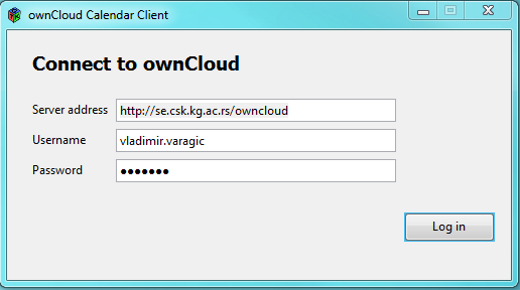
\includegraphics[scale=0.5]{slike/logInForm.png}
	\caption{Форма за пријаву на систем}
	\label{fig:xwt_login_form}
\end{figure}

\section {WebDAV}

\textit{WebDAV} представља проширење постојећег \textit{HTTP} протокола. \textit{WebDAV} протокол обезбеђује окружење које корисницима пружа могућност креирања, ажурирања, преузимања документа са удаљеног сервера. Значајно унапређење које је \textit{WebDAV} протокол донео огледа се у количини података који могу да се преносе путем мреже. Раније је број датотека био ограничен на једну датотеку по упиту, а овим протоколом се омогућава преношење више датотека. Битно својство овог протокола је и то да нуди и контролу верзије података (нпр. одржавање информација о аутору документа, датуму и времену измене документа итд.).

За разлику од других протокола за пренос података (\textit{FTP}, \textit{SSH}) за које је потребно додатно отварање портова, \textit{WebDAV} протокол користи стандардан \textit{HTTP}-порт (обично 80), па додатне конфигурације на нивоу мреже нису потребне.

Што се тиче техничке позадине \textit{WebDAV} протокола, он се састоји из скупа нових метода и заглавља постојећег \textit{HTTP} протокола и највероватније је први протокол који користи \textit{XML} језик. Методе које користи су:
\begin{itemize}
	\item {\textit{PROPFIND} -  користи се за читање особина ресурса као и евентуалне структуре истих},
	\item {\textit{PROPPATCH} - мења и брише више особина ресурса у једном кораку},
	\item {\textit{MKCOL} - креира нову колекцију},
	\item {\textit{COPY} - копира ресурс са једне на другу адресу (URI)},
	\item {\textit{MOVE} - пребацује ресурс са једне на другу адресу (URI)},
	\item {\textit{LOCK} - штити ("закључава") ресурс},
	\item {\textit{UNLOCK} - уклања заштиту ресурса}.
\end{itemize}

Готово сви оперативни системи имају уграђену подршку за \textit{WebDAV} протокол. У следећем примеру приказано је како се помоћу \textit{WebDAV} протокола, коришћењем \textit{PROPFIND} методе преузмa вредност поља \textit{displayName} из документа \textit{test.eml}:
\lstinputlisting[language=csharp,caption=Пример коришћења \textit{PROPFIND} методе \textit{WebDAV} протокола]{primeri_koda/webDAV_example.cs}

\section {CalDAV}

\textit{CalDAV} протокол је проширење \textit{WebDAV} протокола и представља  интернет стандард који омогућава клијенту да приступи информацијама о планираним догађајима на удаљеном серверу. Користи \textit{ICalendar}\cite{ical} формат података. Дозвољава истовремени приступ истим подацима од стране више клијената, чиме се омогућава кооперативно планирање и дељење информација. Дакле, \textit{CalDAV} je клијент/сервер протокол за календар и планирње који омогућава корисницима приступ до календара на серверу и могућност планирања догађаја са другим корисницима сервера. У наставку је дат приказ кода за преузимање информација о догађајима са \textit{OwnCloud} календара, коришћењем \textit{CalDAV} протокола:
\lstinputlisting[language=csharp,caption=Преузимање информација о догађајима са \textit{OwnCloud} календара]{primeri_koda/caldav_get_events.cs}
\chapter{\textit{OwnCloud} пројекат}
\label{chap:ownCloud}

\chapter{Синхронизација календара за \textit{оwnCloud} платформу}
\label{chap:ownCloudCalendarSynchronization}

У претходним поглављима описани су основни концепти технологија и окружења који су коришћени у развоју датог пројекта, са циљем да се читаоцу омогући да формира слику комплетног, заокруженог, решења. Сам пројекат, који је тема овог рада, може се посматрати као део тог решења. У овом поглављу фокус ће бити постављен на појашњења неких делова његове имплементације.

\section{Жељене функционалности}

Актуелна, званична, верзија \textit{оwnCloud} десктоп клијента обезбеђује само синхронизацију докумената који се налазе на \textit{оwnCloud} платформи. Основни циљ овог пројекта јесте да се развије решење, у виду мултиплатформског десктоп клијента, које би омогућило преузимање информација о креираним догађајима на \textit{оwnCloud} календару и приказ одговарајућих обавештења. Апликација има следећи скуп функционалности:
\begin{itemize}
	\item{синхронизација догађаја на захтев},
	\item{аутоматска синхронизација догађаја},
	\item{могућност управљања аутоматском синхронизацијом (потребна/није потребна, дефинисање временског интервала након којег ће се стартовати,...)},
	\item{преглед преузетих догађаја},
	\item{приступ делу за администрацију догађаја на веб порталу \textit{оwnCloud} платформе},
	\item{приказ одговарајућег обавештења, непосредно пре почетка неког догађаја}.	
\end{itemize}

Ток активности које треба да обезбеде ове функционалности описан је на дијаграму \ref{fig:application_alogorithm}.

\begin{figure}[H]
	\centering
	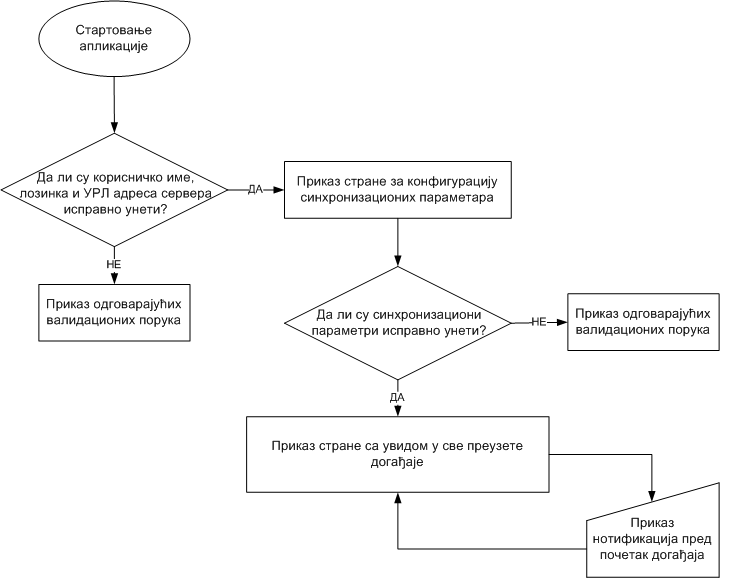
\includegraphics[scale=0.5]{slike/tok_aktivnosti.png}
	\caption{Дијаграм тока активности}
	\label{fig:application_alogorithm}
\end{figure}

На основу приказаног алгоритма  може се стећи јасна и потпуна слика о начину рада саме апликације. У наставку ће бити детаљније објашњене неке интересантније функционалности и биће приказани делови програмског кода, док се комплетан код пројекта може погледати на одговарајућем репозиторијуму\cite{svn_repo}.

\subsection{Аутентификација}

Аутентификација корисника на веб портал \textit{оwnCloud} платформе одрађена је коришћењем класа \textit{WebClient}, \textit{NetworkCredential} које су саставни део \textit{.NET Framework-a}.  Подаци унети на форми за пријаву на систем (Слика \ref{fig:login_form}), која се приказује након стартовања апликације, се прослеђују на верификацију:

\begin{figure}[H]
	\centering
	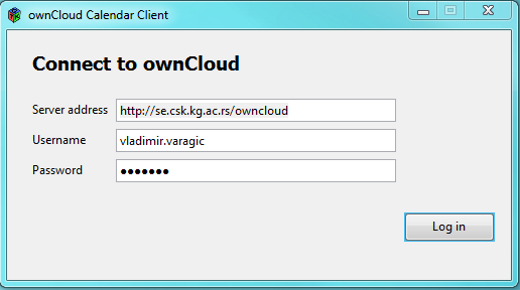
\includegraphics[scale=0.5]{slike/logInForm.png}
	\caption{Форма за пријаву на систем}
	\label{fig:login_form}
\end{figure}

Сви подаци на форми за пријаву су обавезни, па се у случају да неки податак није унет, прикаже одговарајући индикатор:

\begin{figure}[H]
	\centering
	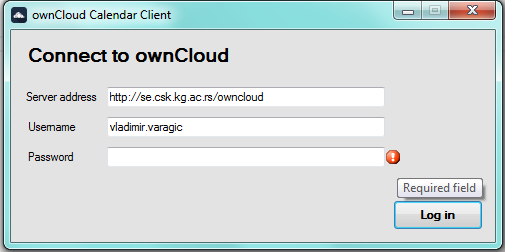
\includegraphics[scale=0.5]{slike/LogInFormReqiredFields.png}
	\caption{Форма за пријаву на систем}
	\label{fig:login_form_required}
\end{figure}

Такође, у случају да неки од података који се уносе приликом пријаве на апликацију (адреса сервера, корисничко име или лозинка) није исправан приказује се одговарајућа порука:

\begin{figure}[H]
	\centering
	\includegraphics[scale=0.5]{slike/logInFailed.png}
	\caption{Форма за пријаву на систем}
	\label{fig:login_form_failed}
\end{figure}

У супротном, ако су сви подаци исправни, корисник успешно приступа апликацији и приказује му се форма за синхронизацију догађаја са \textit{оwnCloud} календара.

\subsection{Синхронизација догађаја на захтев}

Као што је већ наведено у поглављу \textit{5.1.1 Аутентификација}, након успешног приступа апликацији кориснику се приказује форма за конфигурацију синхронизације:

\begin{figure}[H]
	\centering
	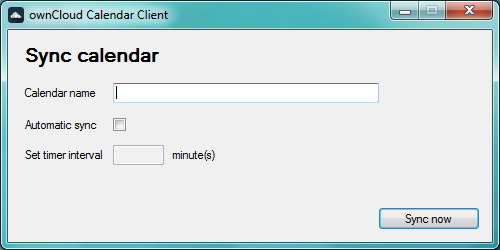
\includegraphics[scale=0.5]{slike/SyncCalendar.png}
	\caption{Синхронизација догађаја са \textit{оwnCloud} календара}
	\label{fig:sync_calendar}
\end{figure}

\textit{OwnCloud} платформа омогућава кориснику да на порталу води више различитих календара тј. да календар дели у различите категорије. 

\begin{figure}[H]
	\centering
	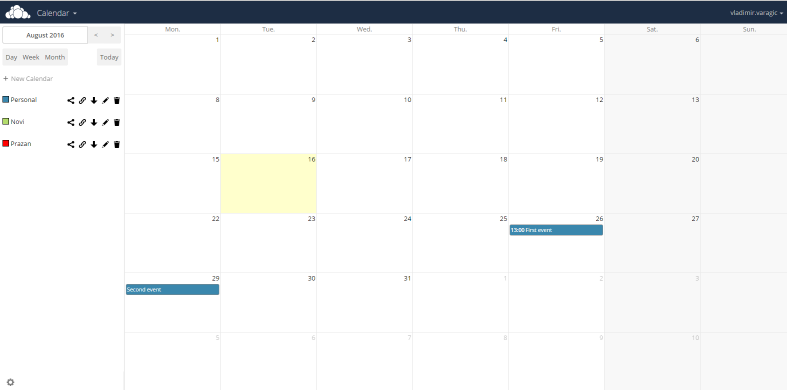
\includegraphics[scale=0.5]{slike/ownCloudCalendar.png}
	\caption{\textit{OwnCloud} календар}
	\label{fig:own_cloud_calendar}
\end{figure}

Са друге стране, синхронизацијом се у једном тренутку могу преузети само догађаји који су везани за једну категорију, тако да је назив календара обавезан податак приликом синхронизације. Такође, приликом покретања синхронизације ради се валидација исправности назива календара и уколико не постоји календар са унетим називом кориснику се прикаже одговарајућа порука. У супротном, ако је унет исправан назив календара, кориснику се приказују догађаји који постоје на наведеном календару. Сам приказ података о догађају биће детаљно описан у секцији \textit{5.1.4 Преглед перузетих догађаја}.

Методе којима се синхронизују подаци приказани су на слици \ref{fig:sync_calendar_method}

\begin{figure}[H]
	\centering
	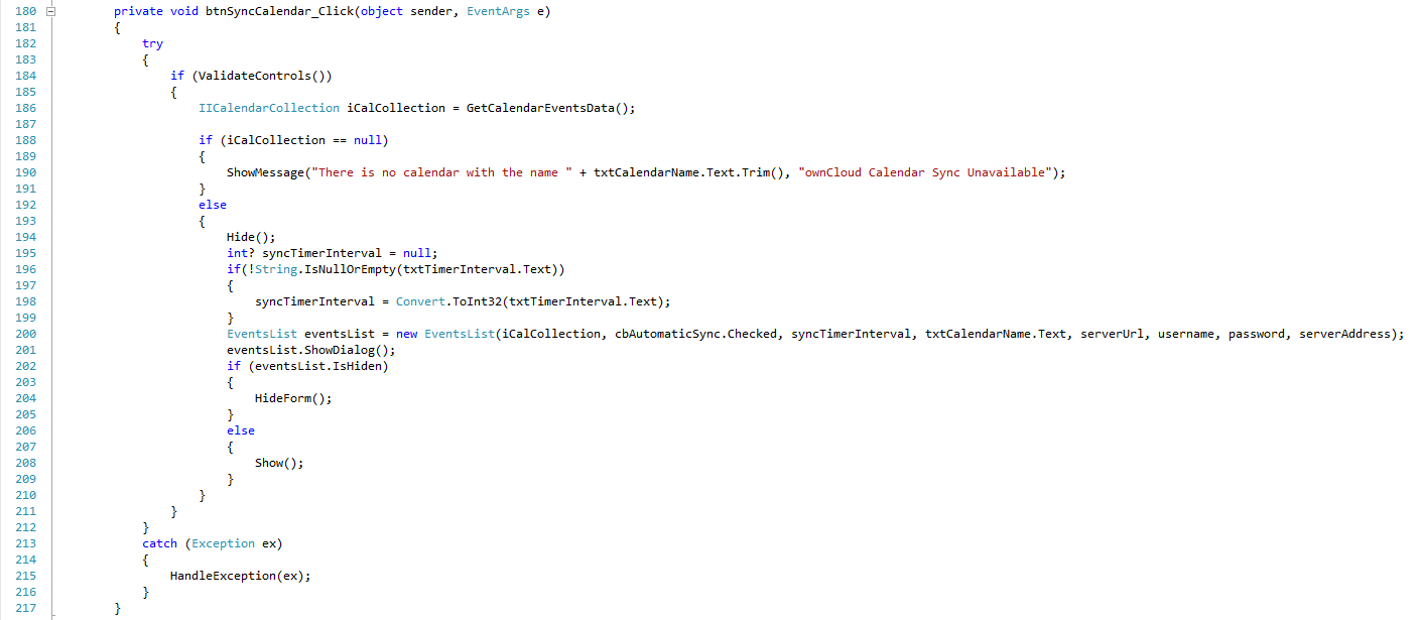
\includegraphics[scale=0.5]{slike/SyncCalendarMethod.png}
	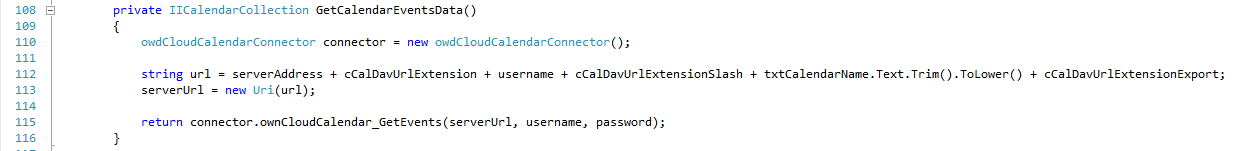
\includegraphics[scale=0.5]{slike/GetCalendarEventsDataMethod.png}
	\caption{Методе за синхронизацију догађаја са \textit{оwnCloud} календара}
	\label{fig:sync_calendar_method}
\end{figure}

\subsection{Аутоматска синхронизација догађаја}

Поред наведене функционалности за синхронизацију догађаја на захтев, омогућена је и функционалност аутоматске синхронизације догађаја. Уколико корисник жели да користи дату функционалност, потребно је да чекира опцију \textit{Automatic sync} на форми за синхронизацију догађаја (Слика \ref{fig:sync_calendar}). Када је опција \textit{Automatic sync} чекирана, податак \textit{Sync time interval} је обавезан. Дакле, након дефинисања наведених података, апликација ће аутоматски синхронизовати догађаје са одговарајућег календара у наведеном временском интервалу. Времески интервал се дефинише у минутима и одговарајућом валидацијом онемогућемо је да вредност овог податка буде било шта што није цео позитиван број.

\subsection{Преглед преузетих догађаја}
Када су сви обавезни подаци исправно унети, било да је у питању синхронизација догађаја на захтев, било да је у питању аутоматска синхронизација догађаја, кликом на дугме \textit{Sync now} (Слика \ref{fig:sync_calendar_personal}) прузимају се догађаји са одговарајућег календара и прикаже се форма са листом догађаја (Слика \ref{fig:events_list}):

\begin{figure}[H]
	\centering
	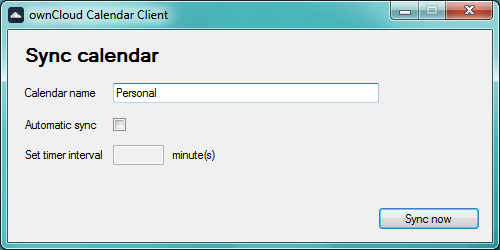
\includegraphics[scale=0.5]{slike/SyncCalendarPersonal.png}
	\caption{Синхронизација догађаја са \textit{оwnCloud} календара}
	\label{fig:sync_calendar_personal}
\end{figure}

\begin{figure}[H]
	\centering
	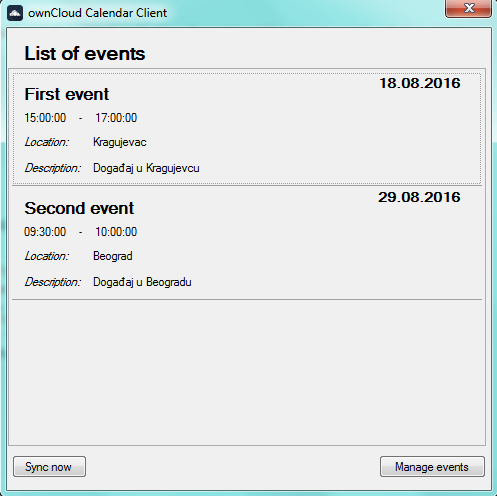
\includegraphics[scale=0.5]{slike/EventsList}
	\caption{Приказ преузетих догађаја}
	\label{fig:events_list}
\end{figure}

Са форме за Преглед преузетих догађаја (Слика \ref{fig:events_list}) корисник у сваком тренутку може поново да покрене синхронизацију догађаја (кликом на дугме \textit{Sync now}), без обзира на то да ли је функционалност аутоматске синхронизације изабрана или не. Корисник, такође, има могућност да са форме за Преглед преузетих догађаја  (Слика \ref{fig:events_list}), кликом на дугме \textit{Manage events} приступи календару на веб порталу \textit{оwnCloud} платформе (Слика \ref{fig:own_cloud_calendar})  и администрира (креира нове, ажурира постојеће, брише) догађаје.

\subsection{Приказ нотификација}

Поред описаних функционалности апликација има још једну, вероватно најзанимљивију функционалност, а то је приказ одговарајућих нотификација у вези са преузетим догађајима. Нотификације се приказују према унапред дефинисаним параметрима:
\begin{itemize}
	\item{први параметар (\textit{notificationMessageTimerInMinutes}) представља временски период (у минутима) којим се дефинише колико минута пре стартовања догађаја приказати одговарајућу нотификацију},
	\item{други параметар (\textit{notificationPingTimeInterval}) представља времески период (у милисекундама) којим се дефинише колико често ће се проверавати да ли је први параметар достигао дефинисану вредност}.	

\end{itemize}
Ови параметри су конфигурабилни и део су конфигурационог фајла:

\begin{figure}[H]
	\centering
	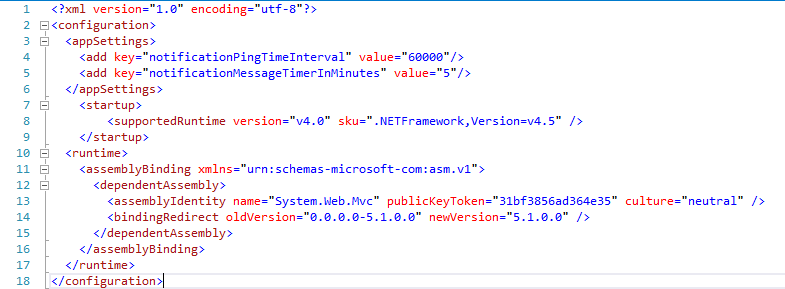
\includegraphics[scale=0.5]{slike/AppConfig.png}
	\caption{Конфигурациони фајлl}
	\label{fig:app_config}
\end{figure}

Дакле, у складу са дефинисаним вредностима наведених параметара, апликација сваког минута проверава да ли постоји догађај који ће стартовати за 5 минута и у случају да такав догађај постоји, кориснику се прикаже одговарајућа нотификација:

\begin{figure}[H]
	\centering
	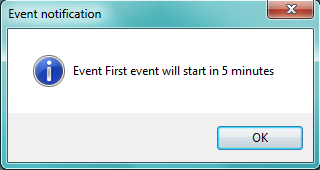
\includegraphics[scale=0.5]{slike/EventNotification.png}
	\caption{Приказ нотификације}
	\label{fig:event_notification}
\end{figure}

У наставку је приказана метода којом је дата функционалност имплементирана:

\begin{figure}[H]
	\centering
	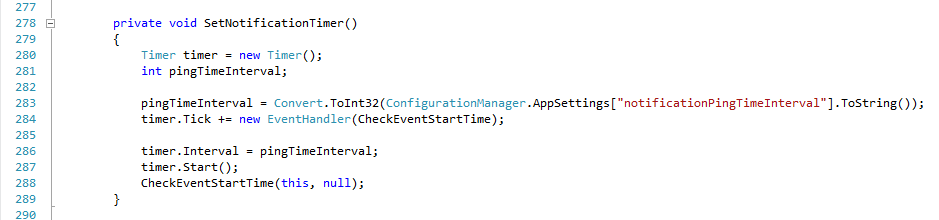
\includegraphics[scale=0.5]{slike/SetNotificationTimer.png}
	\caption{Метода за приказ нотификација}
	\label{fig:set_notification_timer}
\end{figure}

Поред функционалности описаних у претходним секцијама, споменућемо још нека свoјства апликације. Најпре, треба нагласити да је апликација \textit{Single instance}, односно у једном тренутку могуће је покренути само једну инстанцу апликације. У случају да корисник покуша да покрене више инстанци апликације, то му неће бити дозвоњено и приказаће се одговарајућа порука. 
Такође, требало би напоменути да се кликом на дугме \textit{Close} на форми за Приказ преузетих догађаја апликација не затвара, већ се само минимизације, тј. апликација је и даље покренута и иконица апликације налази се у таскбару (Слика \ref{fig:application_icon}):

\begin{figure}[H]
	\centering
	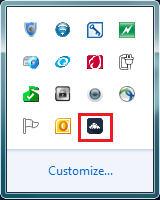
\includegraphics[scale=0.5]{slike/ApplicationIcon.png}
	\caption{Таскбар - приказ иконице}
	\label{fig:application_icon}
\end{figure}

Десни клик на иконицу у таскбару нуди следеће опције (Слика \ref{fig:icon_right_click}):
\begin{itemize}
	\item{отварање форме за приказ преузетих догађаја},
	\item{отварање форме за унос параметара синхронизације},
	\item{одјава са апликације и приказ форме за пријаву},
	\item{затварање апликације}.
\end{itemize}

\begin{figure}[H]
	\centering
	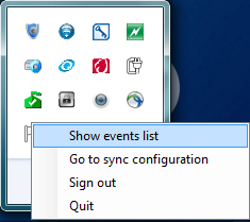
\includegraphics[scale=0.5]{slike/IconRightClick.png}
	\caption{Додатне опције}
	\label{fig:icon_right_click}
\end{figure}

\section{Идеје за даљи развој}

Иако је функционално исправна, постојећу верзију апликације треба посматрати само као полазни корак у развоју коначног производа. Актуелна верзија апликације има својеврсна ограничења условњена коришћеним API-има (нпр. немогућност синронизације више календара истовремено). Унапређења датих API-a или појава нових утицали би на то да се појави потреба за имплементацијом додатних функционалности. Са друге стране, постојећа верзија се такође може унапредити на више начина:
\begin{itemize}
	\item{побољшање корисничког интерфејса},
	\item{предефинисани прикази догађаја (за разлику од актуелног приказа свих догађаја)},
	\item{...}
\end{itemize}
%
% Spisak Literature
%
\begin{thebibliography}{11}
\bibitem{licence} {BSD, GPL и MIT лиценце, \url{http://producingoss.com/en/license-choosing.html}}

\bibitem{git} {GIT, \url{https://git-scm.com/}}

\bibitem{github} {Github, \url{https://github.com/}}

\bibitem{xwt} {XWT платформа, \url{https://github.com/mono/xwt/tree/master/Xwt/Xwt}}

\bibitem{dday} {DDay.iCal - an iCalendar class library, \url{https://sourceforge.net/p/dday-ical/wiki/Home/}}

\bibitem{caldav} {CalDav, \url{http://caldav.calconnect.org/index.html}}

\bibitem{ical} {ICalendar, \url{https://www.calconnect.org/resources/calendaring-standards#iCalendar}}

\bibitem{owncloud} {Званична страница {\it OwnCloud} пројекта, \url{http://owncloud.org/}}

\bibitem{svn_repo} {Репозиторијум {\it ownCloud Calendar Synchronization} апликације, \url{https://own-cloud-calendar.googlecode.com/svn}}

% \bibitem{} {} 
\end{thebibliography}


%
% Koriscenje listinga
%
%\begin{lstlisting}[language=Java,label=lst:rssfeeder,caption=RssItemView.java]
%package pmf.rssfeeder.android;
%
%import android.app.Activity;
%import android.os.Bundle;
%
%public class RssItemView extends Activity
%{
%  /** Called when the activity is first created. */
%  @Override
%  public void onCreate(Bundle savedInstanceState)
%  {
%      super.onCreate(savedInstanceState);
%  }
%}
%\end{lstlisting}
	
\end{document}


